\documentclass[12pt]{article}
\usepackage{graphicx}
\usepackage[none]{hyphenat}
\usepackage{graphicx}
\usepackage{listings}
\usepackage[english]{babel}
\usepackage{graphicx}
\usepackage{caption} 
\usepackage{booktabs}
\usepackage{array}
\usepackage{amssymb} % for \because
\usepackage{amsmath}   % for having text in math mode
\usepackage{extarrows} % for Row operations arrows
\usepackage{listings}
\usepackage[utf8]{inputenc}
\lstset{
  frame=single,
  breaklines=true
}
\usepackage{hyperref}
  
%Following 2 lines were added to remove the blank page at the beginning
\usepackage{atbegshi}% http://ctan.org/pkg/atbegshi
\AtBeginDocument{\AtBeginShipoutNext{\AtBeginShipoutDiscard}}


%New macro definitions
\newcommand{\mydet}[1]{\ensuremath{\begin{vmatrix}#1\end{vmatrix}}}
\providecommand{\brak}[1]{\ensuremath{\left(#1\right)}}
\newcommand{\solution}{\noindent \textbf{Solution: }}
\newcommand{\myvec}[1]{\ensuremath{\begin{pmatrix}#1\end{pmatrix}}}
\providecommand{\norm}[1]{\left\lVert#1\right\rVert}
\providecommand{\abs}[1]{\left\vert#1\right\vert}
\let\vec\mathbf

\begin{document}

\begin{center}
\title{\textbf{VECTORS}}
\date{\vspace{-5ex}} %Not to print date automatically
\maketitle
\end{center}

\section{10$^{th}$ Maths - EXERCISE-7.2}

\begin{enumerate}
\item Find the coordinates of the points of trisection of the line segment joining $\vec(4 ,-1) \text{ and } \vec(-2,-3)$ 
\end{enumerate}

\section{SOLUTION}
Given points are
\begin{align}
\vec{Q}=\myvec{4\\ -1} ,
\vec{P}=\myvec{-2\\ -3}
\end{align}
The equation of the formula is
\begin{align}
\vec{R}=\frac{\vec{Q}+n\vec{P}}{1+n}
\end{align}
Ratio 2:1 has taken 
\begin{align}
n=\frac{1}{2}\\
\vec{R}=\frac{1}{1+\frac{1}{2}}\brak{\myvec{4\\-1}+\frac{1}{2}\myvec{-2\\-3}}\\
\frac{1}{\frac{3}{2}}\brak{\myvec{4\\ -1}+\myvec{-1\\ \frac{-3}{2}}}\\
\frac{1}{\frac{3}{2}}\brak{\myvec{4+-1}\myvec{-1\\ \frac{-3}{2}}}\\
\frac{1}{\frac{}{2}}\brak{\myvec{3 & \frac{-2}{2}}}\\
\frac{3}{\frac{3}{2}}\brak{\frac{\frac{-5}{2}}{\frac{3}{2}}}\\
\vec{R}=\myvec{2 & \frac{-5}{3}}
\end{align}
Ratio 1:2 has taken
\begin{align}
n=\frac{2}{1}\\
\vec{S}=\frac{1}{1+\frac{2}{1}}\brak{\myvec{4\\-1}+\frac{2}{1}\myvec{-2\\-3}}\\
\frac{1}{3}\brak{\myvec{4\\ -1}+\myvec{-4-6}}\\
\frac{1}{3}\brak{\myvec{4+& -4}\myvec{-1+&-6}}\\
\frac{1}{3}\brak{\myvec{0& -7}}\\
\vec{S}=\myvec{0\\ \frac{-7}{3}}
\end{align}
\section{Figure}
\begin{figure}[h]
\centering
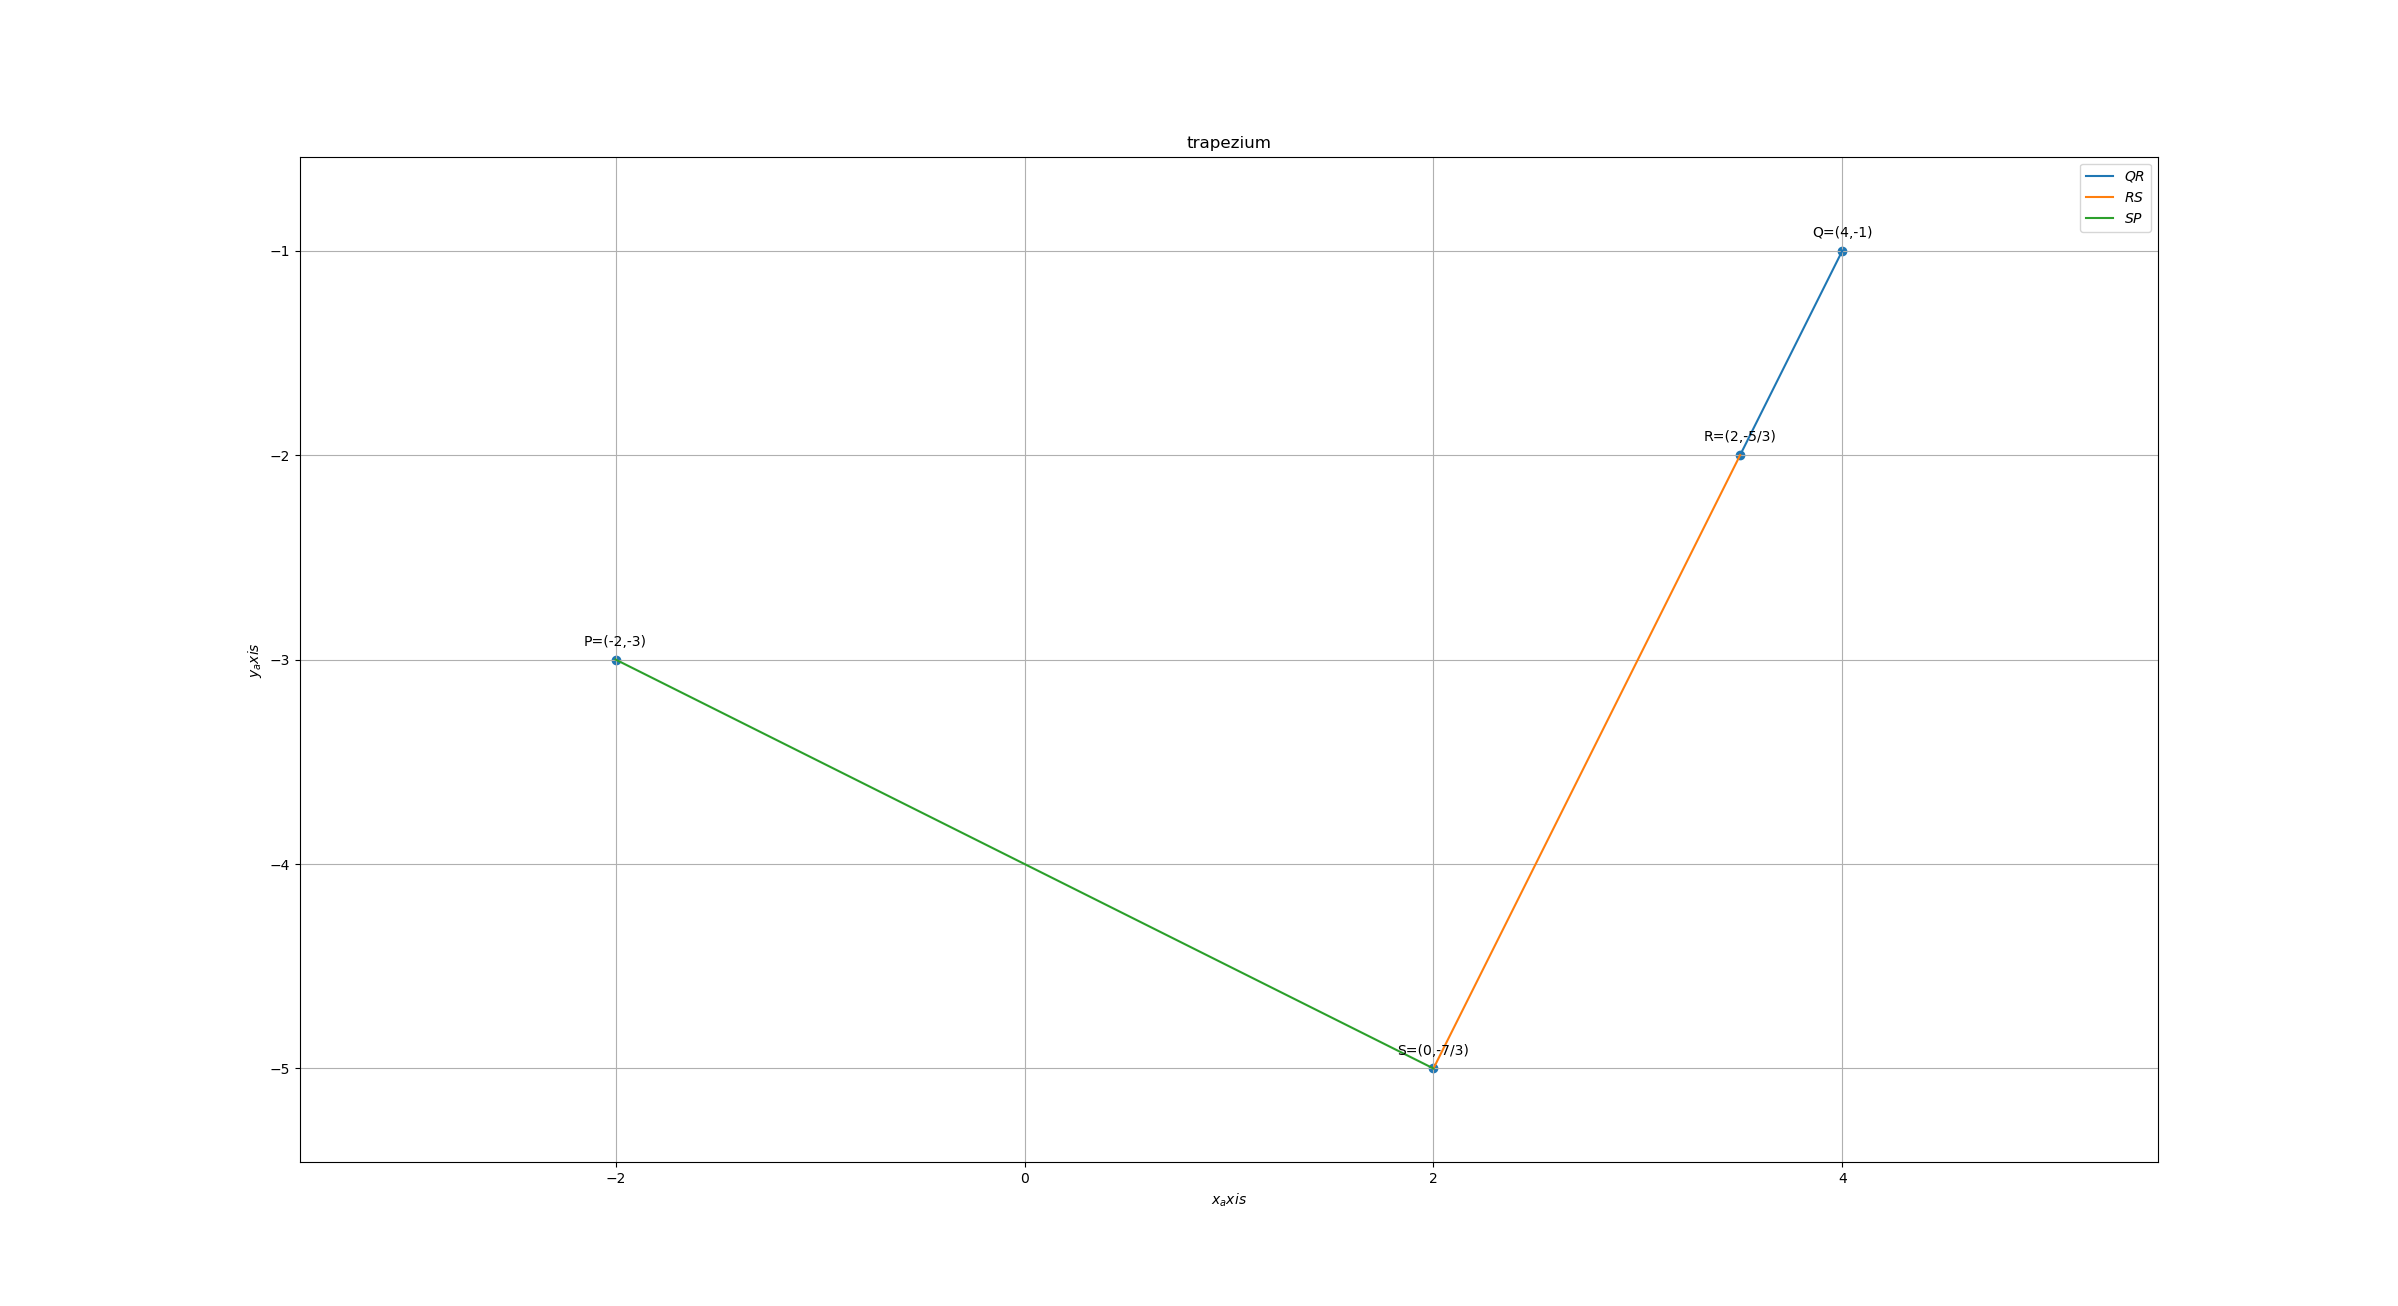
\includegraphics[width=\columnwidth]{vec.png}
\caption{trisecton}
		\label{fig:Figure}
\end{figure}
\begin{lstlisting}
https://github.com/prasaddeva287/FWC/tree/main/VECTORS/7.2/codes
\end{lstlisting}
\end{document}